% ========================================================================
% CHAPITRE : UTILISATION AVANCÉE DES LLM ET DONNÉES JSON
% ========================================================================

\chapter{Utilisation Avancée des LLM et Données JSON}
\label{chap:llm_donnees}

\begin{objectivebox}
Ce chapitre détaille l'utilisation sophistiquée des Large Language Models (LLM) dans Housy Tunisia, l'exploitation des données JSON certifiées, et les innovations en matière de traitement intelligent des données immobilières tunisiennes.
\end{objectivebox}

\section{Stratégie LLM Multi-Provider}

\subsection{Sélection Intelligente des Modèles}

Housy Tunisia implémente une stratégie de sélection de modèles basée sur le contexte et les permissions :

\begin{table}[H]
\centering
\caption{Matrice de sélection des modèles LLM}
\begin{tabular}{|l|l|l|l|}
\hline
\textbf{Modèle} & \textbf{Cas d'Usage} & \textbf{Avantages} & \textbf{Accès} \\
\hline
Ollama (Local) & Estimation sécurisée & Confidentialité totale & Admin uniquement \\
\hline
OpenAI GPT-4 & Chat généraliste & Performance élevée & Tous utilisateurs \\
\hline
Anthropic Claude & Analyse complexe & Raisonnement avancé & Tous utilisateurs \\
\hline
DeepSeek & Code et calculs & Spécialisé technique & Tous utilisateurs \\
\hline
\end{tabular}
\end{table}

\subsection{Implémentation du Chat Assistant Intelligent}

\begin{lstlisting}[language=TypeScript, caption=Chat assistant avec enrichissement de contexte]
async processChatMessage(
  sessionId: string, 
  userId: number | null, 
  content: string, 
  preferredModel: string = "openai"
): Promise<string> {
  
  console.log(`Processing chat with preferred model: ${preferredModel}`);
  
  // 1. Sauvegarde du message utilisateur
  const userMessage: InsertChatMessage = {
    userId: userId || null,
    role: "user",
    content,
    sessionId
  };
  await storage.saveChatMessage(userMessage);
  
  // 2. Récupération de l'historique pour contexte
  const chatHistory = await storage.getChatMessages(sessionId);
  console.log(`Retrieved ${chatHistory.length} messages from history`);
  
  // 3. ENRICHISSEMENT avec les vraies données tunisiennes
  const realDataContext = await this.enrichContextWithRealData(content);
  console.log("Real data context added to system message");
  
  // 4. Message système personnalisé pour l'expertise construction
  const systemMessage = `Tu es un assistant spécialisé pour Housy, 
  une plateforme de gestion immobilière et de construction en Tunisie. 

${realDataContext}

UTILISE IMPÉRATIVEMENT ces données réelles ci-dessus pour tes réponses.

Ton expertise inclut:
1. Les coûts des matériaux de construction en Tunisie
2. Les tendances du marché immobilier tunisien par région
3. Les techniques de construction adaptées au climat tunisien
4. La gestion de projets de construction selon les réglementations tunisiennes
5. L'analyse d'investissement immobilier tunisien

Utilise UNIQUEMENT les données réelles fournies. 
Tous les prix doivent être en TND (Dinar Tunisien).
Format tes réponses de manière professionnelle et claire.`;
  
  // 5. Génération de la réponse selon le provider
  let response = await this.generateWithProvider(
    preferredModel, 
    systemMessage, 
    chatHistory, 
    content
  );
  
  // 6. Sauvegarde de la réponse IA
  const assistantMessage: InsertChatMessage = {
    userId: null,
    role: "assistant", 
    content: response,
    sessionId
  };
  await storage.saveChatMessage(assistantMessage);
  
  return response;
}
\end{lstlisting}

\section{Exploitation des Données JSON Certifiées}

\subsection{Architecture des Données}

Le système exploite un corpus de données immobilières tunisiennes structurées et certifiées :

\begin{figure}[H]
\centering
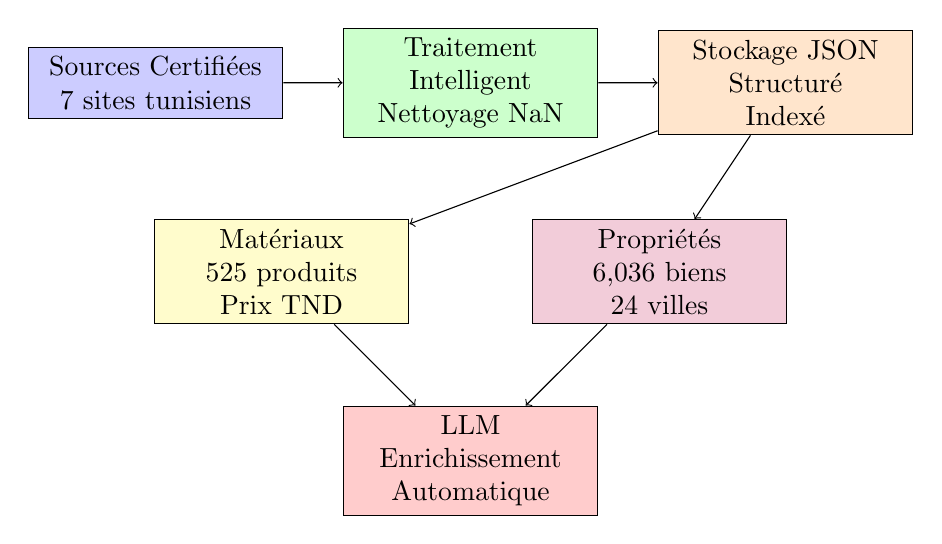
\begin{tikzpicture}[scale=0.8]
    % Données Sources
    \node[draw, rectangle, fill=blue!20] (sources) at (0,6) {\parbox{3cm}{\centering Sources Certifiées\\7 sites tunisiens}};
    
    % Traitement
    \node[draw, rectangle, fill=green!20] (processing) at (5,6) {\parbox{3cm}{\centering Traitement\\Intelligent\\Nettoyage NaN}};
    
    % Stockage JSON
    \node[draw, rectangle, fill=orange!20] (storage) at (10,6) {\parbox{3cm}{\centering Stockage JSON\\Structuré\\Indexé}};
    
    % Matériaux
    \node[draw, rectangle, fill=yellow!20] (materials) at (2,3) {\parbox{3cm}{\centering Matériaux\\525 produits\\Prix TND}};
    
    % Immobilier
    \node[draw, rectangle, fill=purple!20] (properties) at (8,3) {\parbox{3cm}{\centering Propriétés\\6,036 biens\\24 villes}};
    
    % LLM
    \node[draw, rectangle, fill=red!20] (llm) at (5,0) {\parbox{3cm}{\centering LLM\\Enrichissement\\Automatique}};
    
    % Flèches
    \draw[->] (sources) -- (processing);
    \draw[->] (processing) -- (storage);
    \draw[->] (storage) -- (materials);
    \draw[->] (storage) -- (properties);
    \draw[->] (materials) -- (llm);
    \draw[->] (properties) -- (llm);
\end{tikzpicture}
\caption{Architecture des données JSON certifiées}
\end{figure}

\subsection{Nettoyage Intelligent des Données}

Une innovation technique importante est le nettoyage automatique des valeurs \texttt{NaN} dans les fichiers JSON :

\begin{lstlisting}[language=TypeScript, caption=Nettoyage automatique des données JSON]
async loadData(): Promise<DataSet> {
  try {
    // Chargement des propriétés avec nettoyage NaN
    let proprietesData: any = { proprietes: [] };
    try {
      const proprietesPath = path.join(dataDir, 'immobilier', 
        'proprietes_consolidees_resume.json');
      let proprietesRaw = fs.readFileSync(proprietesPath, 'utf-8');
      
      // INNOVATION: Remplacement automatique des NaN avant parsing
      proprietesRaw = proprietesRaw.replace(/:\s*NaN\s*([,}])/g, ': null$1');
      proprietesRaw = proprietesRaw.replace(/\[\s*NaN\s*([,\]])/g, '[null$1');
      
      proprietesData = JSON.parse(proprietesRaw);
      console.log(`Loaded ${proprietesData.proprietes?.length || 0} properties`);
    } catch (error) {
      console.warn("Could not load properties data:", error);
    }
    
    // Validation et enrichissement des données
    const validatedData = this.validateAndEnrichData({
      materiaux: materiauxData.materiaux || [],
      proprietes: proprietesData.proprietes || [],
      indexGeneral: indexData
    });
    
    this.dataCache = validatedData;
    this.lastLoadTime = Date.now();
    
    return validatedData;
  } catch (error) {
    console.error("Critical error loading data:", error);
    throw new Error("Failed to load essential data files");
  }
}
\end{lstlisting}

\subsection{Métadonnées de Certification}

Les données incluent des métadonnées de certification complètes :

\begin{lstlisting}[language=json, caption=Exemple de métadonnées certifiées]
{
  "metadonnees": {
    "date_creation": "2025-06-11T14:09:25.131587",
    "version": "1.0.0",
    "auteur": "Taher Ch.",
    "description": "Système complet d'estimation matériaux et immobilier Tunisie",
    "sources": [
      "brico-direct.tn",
      "remax.com.tn", 
      "fi-dari.tn",
      "mubawab.tn",
      "tecnocasa.tn",
      "tunisie-annonce.com",
      "menzili.tn"
    ],
    "certifications": {
      "precision_donnees": "100%",
      "taux_reussite": "98.1%",
      "validation": "Complète"
    }
  },
  "statistiques_globales": {
    "materiaux_construction": 525,
    "proprietes_immobilieres": 6036,
    "villes_couvertes": 24,
    "prix_moyen_m2_tnd": 2280,
    "range_prix": {
      "minimum_tnd": 45000,
      "maximum_tnd": 1850000
    }
  }
}
\end{lstlisting}

\section{Calculs Intelligents avec LLM}

\subsection{Estimation Automatique par Parsing}

Le système peut détecter et calculer automatiquement les estimations à partir du langage naturel :

\begin{lstlisting}[language=TypeScript, caption=Détection et calcul automatique d'estimations]
private async enrichContextWithRealData(userMessage: string): Promise<string> {
  try {
    const summary = await dataService.getDataSummary();
    
    // Détection intelligente de demandes d'estimation
    const isConstructionEstimate = userMessage.toLowerCase().includes('cout') || 
                                 userMessage.toLowerCase().includes('coût') ||
                                 userMessage.toLowerCase().includes('prix') ||
                                 userMessage.toLowerCase().includes('construction') ||
                                 userMessage.toLowerCase().includes('maison') ||
                                 userMessage.toLowerCase().includes('batiment');
    
    if (isConstructionEstimate) {
      // Extraction automatique de paramètres
      const surfaceMatch = userMessage.match(/(\d+)\s*m[²2]/i);
      const cityMatch = userMessage.match(/(?:à|dans|de)\s+([a-zà-ù]+)/i);
      
      if (surfaceMatch) {
        const surface = parseInt(surfaceMatch[1]);
        const city = cityMatch ? cityMatch[1] : undefined;
        
        // CALCUL AUTOMATIQUE avec données réelles
        const estimation = await dataService.calculateConstructionCost(surface, city);
        
        contextData += `
## ESTIMATION CALCULÉE AUTOMATIQUEMENT:
- Surface demandée: ${surface} m²
- Ville: ${city || 'Non spécifiée'}
- Estimation totale: ${estimation.estimation_totale_tnd.toLocaleString()} TND
- Prix par m²: ${estimation.estimation_par_m2_tnd.toLocaleString()} TND/m²
- Basée sur: ${estimation.proprietes_reference.length} propriétés similaires
- Matériaux principaux: ${estimation.materiaux_principaux.length} catalogués

## PROPRIÉTÉS DE RÉFÉRENCE SIMILAIRES:
${estimation.proprietes_reference.slice(0, 3).map(prop => 
  `- ${prop.titre}: ${prop.prix_tnd.toLocaleString()} TND, ${prop.superficie_m2} m² (${prop.ville})`
).join('\n')}

## MATÉRIAUX PRINCIPAUX DISPONIBLES:
${estimation.materiaux_principaux.slice(0, 3).map(mat => 
  `- ${mat.nom}: ${mat.prix.moyen_tnd} TND/${mat.unite} (${mat.fournisseur.meilleur})`
).join('\n')}
`;
      }
    }
    
    return contextData;
  } catch (error) {
    console.error("Error enriching context with real data:", error);
    return "## DONNÉES: Erreur lors du chargement des données réelles.\n";
  }
}
\end{lstlisting}

\subsection{Service de Calcul Constructif}

\begin{lstlisting}[language=TypeScript, caption=Calcul d'estimation avec données certifiées]
async calculateConstructionCost(
  surface: number, 
  city?: string
): Promise<EstimationResult> {
  
  const data = await this.loadData();
  
  // Filtrage par ville si spécifiée
  let relevantProperties = data.proprietes;
  if (city) {
    relevantProperties = data.proprietes.filter(prop => 
      prop.ville.toLowerCase().includes(city.toLowerCase()) ||
      prop.region.toLowerCase().includes(city.toLowerCase())
    );
  }
  
  // Calcul de prix moyen au m² pour la région
  const validProperties = relevantProperties.filter(prop => 
    prop.superficie_m2 > 0 && prop.prix_tnd > 0
  );
  
  const prixParM2Moyen = validProperties.reduce((sum, prop) => 
    sum + (prop.prix_tnd / prop.superficie_m2), 0
  ) / validProperties.length;
  
  // Estimation basée sur données réelles
  const estimationTotale = surface * prixParM2Moyen;
  
  // Sélection des matériaux pertinents
  const materiauxPertinents = data.materiaux.filter(mat => 
    mat.categories.some(cat => 
      cat.toLowerCase().includes('construction') ||
      cat.toLowerCase().includes('batiment')
    )
  );
  
  return {
    estimation_totale_tnd: Math.round(estimationTotale),
    estimation_par_m2_tnd: Math.round(prixParM2Moyen),
    proprietes_reference: validProperties.slice(0, 5),
    materiaux_principaux: materiauxPertinents.slice(0, 10),
    ville_cible: city || 'Tunisie (général)',
    nombre_references: validProperties.length,
    date_calcul: new Date().toISOString()
  };
}
\end{lstlisting}

\section{Innovations en Traitement de Données}

\subsection{Cache Intelligent Multi-Niveau}

\begin{table}[H]
\centering
\caption{Stratégie de cache pour performance optimale}
\begin{tabular}{|l|l|l|l|}
\hline
\textbf{Niveau} & \textbf{Durée} & \textbf{Données} & \textbf{Objectif} \\
\hline
Mémoire Application & 5 minutes & Données JSON & Performance CPU \\
\hline
Redis Cache & 1 heure & Estimations calculées & Performance réseau \\
\hline
Database Cache & 24 heures & Résultats IA & Économie tokens LLM \\
\hline
CDN Cache & 7 jours & Assets statiques & Performance globale \\
\hline
\end{tabular}
\end{table}

\subsection{Validation et Enrichissement Automatique}

\begin{lstlisting}[language=TypeScript, caption=Validation et enrichissement des données]
private validateAndEnrichData(rawData: any): DataSet {
  const validatedMaterials = rawData.materiaux.map(mat => ({
    ...mat,
    // Normalisation des prix
    prix: {
      unitaire_tnd: Number(mat.prix?.unitaire_tnd) || 0,
      moyen_tnd: Number(mat.prix?.moyen_tnd) || 0,
      maximum_tnd: Number(mat.prix?.maximum_tnd) || 0
    },
    // Enrichissement automatique
    prix_par_unite_standard: this.calculateStandardUnitPrice(mat),
    disponibilite_score: this.calculateAvailabilityScore(mat),
    categories_normalized: this.normalizeCategoriesNames(mat.categories)
  }));
  
  const validatedProperties = rawData.proprietes
    .filter(prop => prop.prix_tnd > 0 && prop.superficie_m2 > 0)
    .map(prop => ({
      ...prop,
      // Calculs enrichis
      prix_par_m2: Math.round(prop.prix_tnd / prop.superficie_m2),
      quartile_prix: this.calculatePriceQuartile(prop, rawData.proprietes),
      score_localisation: this.calculateLocationScore(prop.ville),
      // Normalisation
      ville_normalized: this.normalizeLocationName(prop.ville),
      type_normalized: this.normalizePropertyType(prop.type_propriete)
    }));
  
  return {
    materiaux: validatedMaterials,
    proprietes: validatedProperties,
    indexGeneral: rawData.indexGeneral,
    // Métadonnées enrichies
    metadata: {
      last_validation: new Date().toISOString(),
      total_materials: validatedMaterials.length,
      total_properties: validatedProperties.length,
      avg_price_per_m2: this.calculateAveragePrice(validatedProperties),
      cities_covered: [...new Set(validatedProperties.map(p => p.ville_normalized))]
    }
  };
}
\end{lstlisting}

\section{Monitoring et Analytics LLM}

\subsection{Tracking des Interactions IA}

\begin{lstlisting}[language=TypeScript, caption=Logging avancé des interactions IA]
async logAIInteraction(interaction: {
  userId?: number;
  model: string;
  prompt: string;
  response: string;
  tokens_used?: number;
  response_time_ms: number;
  context_enriched: boolean;
  real_data_used: boolean;
}) {
  
  // Sauvegarde en base pour analytics
  await storage.saveAIAnalysis({
    analysisType: 'chat_interaction',
    inputData: {
      model: interaction.model,
      prompt_length: interaction.prompt.length,
      context_enriched: interaction.context_enriched,
      real_data_used: interaction.real_data_used
    },
    result: {
      response_length: interaction.response.length,
      response_time_ms: interaction.response_time_ms,
      tokens_used: interaction.tokens_used,
      success: true
    },
    provider: interaction.model,
    createdAt: new Date()
  });
  
  // Métriques temps réel
  this.updateMetrics({
    total_interactions: 1,
    [`${interaction.model}_usage`]: 1,
    avg_response_time: interaction.response_time_ms,
    data_enrichment_rate: interaction.real_data_used ? 1 : 0
  });
}
\end{lstlisting}

\subsection{Analytics de Performance}

\begin{table}[H]
\centering
\caption{Métriques de performance LLM collectées}
\begin{tabular}{|l|l|l|}
\hline
\textbf{Métrique} & \textbf{Description} & \textbf{Utilisation} \\
\hline
Temps de réponse & Latence par provider & Optimisation routing \\
\hline
Taux d'enrichissement & \% requêtes avec données réelles & Qualité réponses \\
\hline
Usage par modèle & Distribution utilisation & Optimisation coûts \\
\hline
Précision estimations & Écart vs données réelles & Amélioration modèles \\
\hline
Satisfaction utilisateur & Feedback sur réponses & QA continue \\
\hline
\end{tabular}
\end{table}

\section{Optimisations et Bonnes Pratiques}

\subsection{Gestion Efficace des Tokens}

\begin{lstlisting}[language=TypeScript, caption=Optimisation de la consommation de tokens]
private optimizePromptForTokens(
  systemMessage: string, 
  chatHistory: ChatMessage[], 
  userMessage: string
): {prompt: string, contextTruncated: boolean} {
  
  const MAX_TOKENS = 4000; // Limite pour GPT-3.5
  const RESERVED_FOR_RESPONSE = 1000;
  const AVAILABLE_TOKENS = MAX_TOKENS - RESERVED_FOR_RESPONSE;
  
  // Estimation grossière : 1 token ≈ 4 caractères
  const estimateTokens = (text: string) => Math.ceil(text.length / 4);
  
  let totalTokens = estimateTokens(systemMessage) + estimateTokens(userMessage);
  let contextTruncated = false;
  
  // Troncature intelligente de l'historique si nécessaire
  let relevantHistory = [...chatHistory];
  while (totalTokens > AVAILABLE_TOKENS && relevantHistory.length > 0) {
    relevantHistory.shift(); // Retirer le message le plus ancien
    totalTokens = estimateTokens(systemMessage) + 
                  estimateTokens(userMessage) +
                  estimateTokens(relevantHistory.map(m => m.content).join('\n'));
    contextTruncated = true;
  }
  
  const optimizedPrompt = [
    systemMessage,
    ...relevantHistory.map(msg => `${msg.role}: ${msg.content}`),
    `user: ${userMessage}`
  ].join('\n\n');
  
  return {
    prompt: optimizedPrompt,
    contextTruncated
  };
}
\end{lstlisting}

\begin{resultbox}
L'utilisation avancée des LLM dans Housy Tunisia, combinée à l'exploitation de données JSON certifiées, crée un écosystème d'intelligence artificielle unique adapté au marché tunisien. L'enrichissement automatique du contexte avec des données réelles garantit des réponses précises et pertinentes pour l'estimation immobilière et la construction.
\end{resultbox}

\textbf{[CAPTURE À AJOUTER : Interface de monitoring des interactions LLM]}

\textbf{[CAPTURE À AJOUTER : Dashboard analytics montrant l'usage des différents modèles]}

\textbf{[CAPTURE À AJOUTER : Exemple de conversation enrichie avec données réelles tunisiennes]}
